\cleardoublepage

\newrefsection

\chapter{外文翻译}
\sectionnonum{摘要}
在本文中,我们介绍了 OminiControl,这是一种高度通 用且参数高效的框架,它将图像条件集成到预先训练的扩散transformer (DiT) 模型中。\
 OminiControl 的核心是利用参数重用机制,使 DiT 能够使用自身作为强大的骨干对图像条件进行编码,并使用其灵活的多模式注意处理器来处理它们。\
 与严重依赖具有复杂架构的附加编码器模块的 现有方法不同,Omini-Control 有效且高效地结合了注入图像条件,仅需要 0.1\% 的附加参数,并且以统一的方式解决广泛的图像调节任务.\
 方式包括主题驱动的生成和空间对齐条件,例如边缘、深度图等。值得注意的是,这些能力是通过对DiT本身生成的图像进行训练来实现的,这对于主题驱动的生成特别有利。广泛的评估表明,\
 OminiControl 在主题驱动和空间对齐条件生成方面均优于现有的基于 UNet 和 DiT 的模型。此外, 我们还发布了训练数据集,Subjects200K,这是一个包含超过 200,000 个身份一致图像的多样化集合,\
 以及一个高效的数据合成pipeline,以推进主题一致生成的研究。
\begin{figure}[htbp]
    \centering
    \includegraphics[width=0.8\textwidth]{main_cvpr.pdf}
    \caption{OminiControl在主体驱动任务和空间对齐任务上的实验结果。小红框里面展示的是输入条件。}
    \label{fig:example}
  \end{figure}
\section{简介}
扩散模型彻底改变了视觉生成领域,在图像质量 和多样性方面表现出显着优于生成对抗网络(GAN)\cite{heusel2017gans} 等传统方法的卓越能力。虽然这些模型擅长生成高度逼真 的图像,但仍然存在一个关键的挑战:实现对通用模型的 精确和灵活的控制。\
基于文本的调节一直是推进可控生成的基石,为用户提供直观的界面来指定他们期望的输出。然而,仅文本提示通常无法传达用户希望控制的精确空间细节和结构属性。 因此,最近的研究探索了指导扩散模型的互补调节模式,其中基于图像的控制成为一种特别有效的方法。\
这种多模态调节策略可以对生成过程进行更详细和准确的控制,解决纯文本界面固有的局限性。当前的图像调节方法可以大致分为空间对齐和非空间对齐方法。空间对齐的任务(例如草图到图像和修复)需要调节与输出图像之间的直接对应,通常通过 ControlNet\cite{li2025controlnet} 等方法来实现,\
这些方法以空间保留的方式注入调节特征。相比之下,非空间对齐的应用程序,包括主题驱动的生成和风格转移,如 IP-Adapter\cite{ye2023ip} 所示,通常采用像 CLIP 这样的预训练编码器来提取全局特征, 以便通过交叉注意机制进行集成。尽管现有图像条件方法的有效性,但它们存在一些限制,阻碍了它们的效率和灵活性。\
首先,大多数现有方法都是专门为基于UNet的体系结构设计的\cite{li2025controlnet,peng2024controlnext,mou2024t2i,ronneberger2015u,ruiz2023dreambooth},如稳定扩散模型中所示。虽然这些方法与 UNet 的编码器-解码器结构配合良好,但它们可能无法有效地转换为更先进的扩散变换器 (DiT) 模型,而后者已证明了卓越的图像生成质量\cite{chen2023pixart}。此外,当前的方法通常专注于空间对齐的任务或非空间对齐的任务,缺乏有效处理这两种控制类型的统一架构。\
这一局限性通常要求从业者针对不同的控制场景采用不同的方法,增加了系统复杂性和实现开销。此外,这些方法严重依赖额外的网络结构\cite{li2024photomaker,mou2024t2i,ye2023ip,zhang2023adding,zhang2024ssr,qin2023unicontrol}, 这会引入大量的参数开销。为了解决这些限制, 我们提出了一种参数有效的方法,将基于图像的控制合并到 DiT 架构中。我们的方法重用模型现有的 VAE 编码器\cite{rombach2022high} 来处理调节图像。遵循与噪声图像标记相同的标记处理管道,我们使用可学习的位置嵌入来增强编码特征,\
并将它们与潜在噪声无缝集成去噪网络。这个设计实现整个 DiT 块中条件标记和生成标记之间的直接多模态注意交互(MM-Attention)\cite{peebles2023scalable,ruan2023mm},促进高效的信息交换和控制信号传播。我们在高性能 DiT 结构扩散模型 FLUX.Θ-dev 上实现了我们的方法\cite{blackforestlabs_flux}, 一个包含120亿个参数的大规模模型, 并在边缘引导生成、深度感知合成、区域特定编辑和身份保留生成等领域展开了的广泛实验, 
与基于 UNet 的实现和他们在 FLUX模型上的其他应用\cite{flux1controlnet2024}进行比较,都取得了较优的结果。我们还开发了一种新颖的数据合成架构,可以生成高质量、身份一致的图像对。使用此架构,我们创建了一个包含超过 200,000 个不同图像的综合数据集。\
为了促进这个方向的未来研究,我们将发布我们的数据集和完整的网络架构实现作为开源资源。总之,我们的贡献如下:1。我们提出了一种参数有效的方法,用于在扩散Transformer(DiT)模型中实现图像条件控制,在统一的框架内实现空间对齐和非空间对齐控制。2.我们通过跨不同控制任务(包括边缘引导生成、深度感知合成、区域特定编辑和身份保留生成)的广泛实验证明了我们方法的有效性。3.我们开发并发布了Subjects200K数据集,一个包含超过200,000张主题一致图像的高质量数据集,以及高效的数据合成方式,为相关研究进一步探索主题一致的生成任务提供了宝贵的资源。
\section{相关文章}
\subsection{Diffusion模型}
基于扩散的方法已成为图像生成的强大框架\cite{ho2020denoising,rombach2021highresolution},在各种任务中都卓有成效,包括文本到图像合成、图像到图像翻译和图像编辑。最近Diffusion模型的快速发展使得模型生成图片的质量和效率的显著提高。\
为了进一步增强生成能力,大规模 Transformer 架构已集成到这些框架中,从而产生了 DiT 等复杂模型。基于这些架构创新, FLUX包含flow-matching方法达到了SOTA效果。
\begin{figure}[htbp]
    \centering
    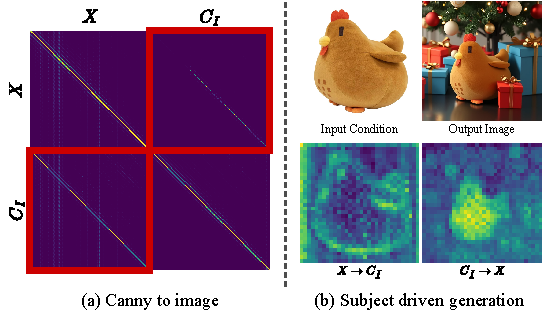
\includegraphics[width=0.8\textwidth]{attn.pdf}
    \caption{(a)线条图到图像任务的注意力图,展示了噪声图像token和参考图像token之间联系。(b)针对主体驱动任务,给定输入条件和输出图片。分别计算的注意力图展现了很精确的主体特征。}
    \label{fig2}
\end{figure}
\subsection{利用diffusion模型进行可控生成}
可控生成在扩散模型的背景下得到了广泛的研究。 文本到图像模型为条件生成奠定了基础, 同时已经开发出各种方法来合并图像等附加控制信号。值得注意的方法包括 ControlNet\cite{zavadski2023controlnet}(在扩散模型中实现空间对齐控制)和 T2I-Adapter\cite{mou2024t2i}通过轻量级适配器提高效率)。 UniControl\cite{zhao2024uni}使用 Mixture-of-Experts (MoE) 来统一不同的空间条件,进一步减小模型大小。\
然而,这些方法依赖于在空间上向去噪网络的隐藏状态添加条件信息,本质上限制了它们对非空间任务(如主题驱动生成)的有效性。 IP-Adapter\cite{ye2023ip}通过额外的编码器引入交叉注意力来解决这个问题,而SSREncoder\cite{zhang2024ssr}进一步增强了图像条件任务中的身份保护。尽管取得了这些进步,但空间对齐和非对齐任务的统一解决方案仍然难以实现。
\section{方法}
\subsection{前置条件}
\begin{figure}[htbp]
    \centering
    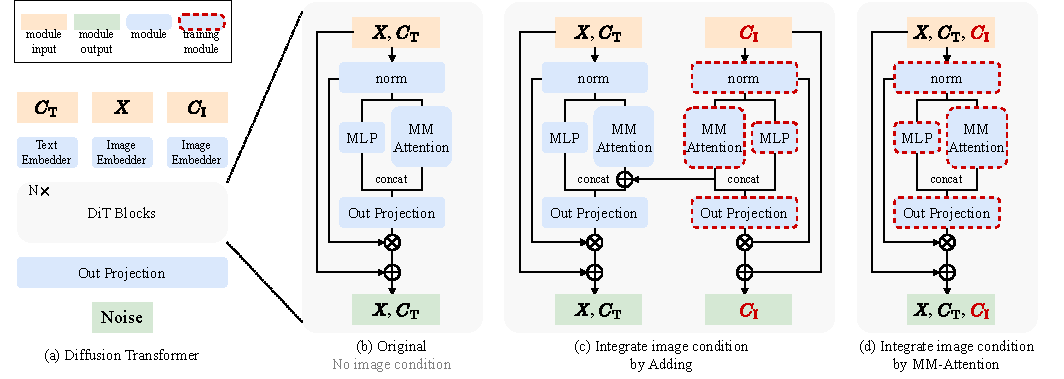
\includegraphics[width=0.8\textwidth]{MainPipe.pdf}
    \caption{DiT架构和有参考图条件的结合架构总览}
    \label{fig3}
\end{figure}
Diffusion Transformer (DiT) 模型 \cite{peebles2023scalable} 在 FLUX-$\Theta$ \cite{blackforestlabs_flux}、Stable Diffusion 3 \cite{esser2024scaling} 和 PixArt \cite{chen2023pixart} 等架构中被广泛采用,其核心是通过Transformer块构建的去噪网络迭代细化噪声图像标记。\
每个Transformer块处理两种类型的标记:噪声图像标记 $\mathbf{X} \in \mathbb{R}^{N \times d}$ 和文本条件标记 $\mathbf{C}_T \in \mathbb{R}^{M \times d}$,其中$d$为嵌入维度,$N$和$M$分别表示图像与文本标记的数量。\
这些标记被映射为隐藏状态$\mathbf{X}'$和$\mathbf{C}_T'$并保持维度一致性。在标准化处理后,核心MM-Attention模块通过旋转位置嵌入(RoPE)\cite{lazos2005rope}整合空间位置信息:\
对于2D网格中的图像标记位置$(i,j)$,RoPE将旋转矩阵$\mathbf{R}(i,j) \in \mathbb【{R}^{d \times d}$作用于查询和键投影,即$\mathbf{Q}_{(i,j)} = \mathbf{W}_Q\mathbf{X}'_{(i,j)} \cdot \mathbf{R}(i,j)$与$\mathbf{K}_{(i,j)} = \mathbf{W}_K\mathbf{X}'_{(i,j)} \cdot \mathbf{R}(i,j)$,\
而文本标记位置在FLUX-$\Theta$中固定为$(0,0)$。随后,图像与文本的查询、键、值被连接为统一矩阵$\mathbf{Q}_Z = [\mathbf{Q}_X; \mathbf{Q}_{C_T}]$,$\mathbf{K}_Z = [\mathbf{K}_X; \mathbf{K}_{C_T}]$,$\mathbf{V}_Z = [\mathbf{V}_X; \mathbf{V}_{C_T}]$,\
构成组合标记集$\mathbf{Z} = [\mathbf{X}; \mathbf{C}_T]$。跨模态交互通过注意力计算实现:
\begin{equation}
    \text{Attention}(\mathbf{Q}_Z, \mathbf{K}_Z, \mathbf{V}_Z) = \text{softmax}\left(\frac{\mathbf{Q}_Z\mathbf{K}_Z^T}{\sqrt{d}}\right)\mathbf{V}_Z
\end{equation}该机制有效融合了视觉特征与语义条件,驱动生成过程。
\subsection{融入图像条件}
我们的方法首先通过预训练VAE对条件图像进行编码,将其投影到与噪声图像标记同构的潜在空间形成条件图像标记$\mathbf{C}_I \in \mathbb{R}^{N \times d}$。传统方法如ControlNet \cite{li2025controlnet}和T2I-Adapter \cite{mou2024t2i}通过空间对齐将条件图像隐藏状态$\mathbf{H}_{C_I}$直接叠加到噪声图像标记:
\begin{equation}
    \mathbf{H}_X = \mathbf{X} + \mathbf{H}_{C_I}
\end{equation}
其中$\mathbf{H}_X$表示组合后的隐藏状态。虽然该范式在空间对齐任务(如姿态控制)中有效,但面临双重局限:(1) 无法处理非对齐控制场景(如文本引导的局部编辑),(2) 即使空间对齐,简单的状态叠加会约束标记间细粒度交互,抑制模型表达能力。为此,我们提出将条件图像标记$\mathbf{C}_I$与噪声图像标记$\mathbf{X}$、文本条件标记$\mathbf{C}_T$统一整合为序列:
\begin{equation}
    \mathbf{Z} = [\mathbf{X}; \mathbf{C}_T; \mathbf{C}_I] \in \mathbb{R}^{(N+M+K) \times d}
\end{equation}
通过多模态注意力机制实现跨标记交互。相比直接相加,该方法在生成质量和条件匹配度上均显著优于基线,且训练曲线表现出更快的收敛速度与更低的重建损失。此外,这种统一序列方法的有效性在空间对齐和非空间对齐任务中得到了证明,突出了其在处理不同条件生成场景方面的多功能性。
\subsection{自适应位置嵌入}
我们的统一的模型设计允许灵活的集成条件图像标记,但前提是需要合并位置信息以确保与噪声图像标记的有效交互。这些tokens的相对位置定位至关重要,因为它直接影响模型的学习效率和泛化能力。在FLUX的 Transformers中,每个token都被分配一个对应的位置索引来编码空间信息。对于512×512的目标图像,VAE编码器首先将其投影到潜在空间中, \
然后将潜在表示划分为 32×32 的标记网格,其中每个token被分配一个唯一的二维位置索引(i, j),其中 i, j $\in$ [0, 31]。这种索引方案保留了潜在空间中原始图像的空间结构。文本标记则保持固定的位置索引 (0, 0)。对于空间对齐的任务,我们最初的方法是为条件标记分配与其对应标记相同的位置嵌入。然而,对于非空间对齐的任务(例如主体驱动生成),\
我们的实验表明,改变条件标记的位置索引会导致更快的收敛。具体来说,我们将条件图像标记转移到索引 (i, j),其中 i $\in$ [0, 31] 和 j $\in$ [32, 64],确保与原始图像标记 X 没有空间重叠。
\subsection{强度系数}
为实现条件图像影响力的动态调控,我们提出可微调节机制:在推理阶段通过强度因子$\gamma \in [0, +\infty)$控制条件效应。当$\gamma=0$时完全消除条件影响,输出退化为原始输入引导结果;$\gamma=1$保持标准条件强度;$\gamma>1$时条件特征显著增强。该功能通过在MM-Attention中引入\textbf{可学习偏置项}实现,将原始注意力计算式(3)扩展为:
\begin{equation}
    \text{Attention}(\mathbf{Q}_Z, \mathbf{K}_Z, \mathbf{V}_Z) = \text{softmax}\left(\frac{\mathbf{Q}_Z\mathbf{K}_Z^T}{\sqrt{d}} + \mathbf{B}(\gamma)\right)\mathbf{V}_Z
\end{equation}
其中偏置矩阵$\mathbf{B}(\gamma) \in \mathbb{R}^{(M+\varepsilon N)\times(M+\varepsilon N)}$结构设计如下:
\begin{equation}
    \mathbf{B}(\gamma) = \begin{bmatrix}
        \mathbf{0}_{M \times M} & \mathbf{J}_{M \times N} \\
        \mathbf{J}_{N \times M} & \log(\gamma) \cdot \mathbf{I}_{N \times N}
    \end{bmatrix}
\end{equation}
这里$M$为文本标记数,$N$为图像相关标记数,$\mathbf{J}$表示全1矩阵,$\mathbf{I}$为单位矩阵。该设计确保文本标记自注意力保持原始模式,图像-条件交互强度由$\log(\gamma)$线性调控,文本-图像交叉注意力通过全1矩阵维持基础关联。

\begin{figure}[htbp]
    \centering
    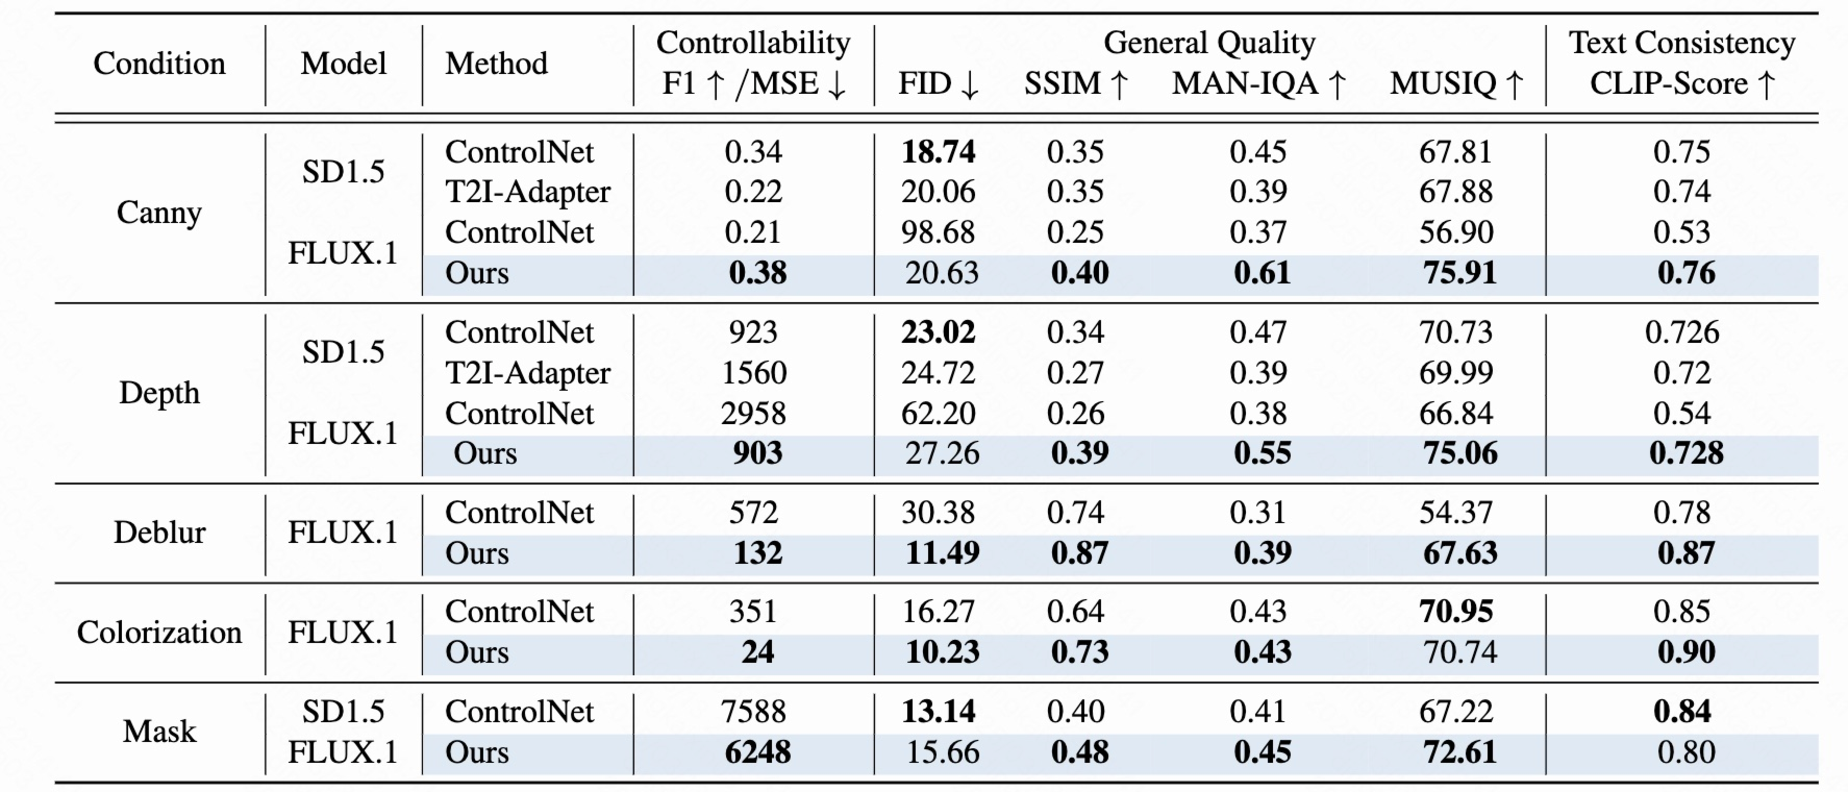
\includegraphics[width=0.8\textwidth]{table.pdf}
    \caption{实验结果表格}
    \label{fig:table}
\end{figure}
\subsection{Subject200K数据集}
用于主体一致生成的训练模型通常需要相同主体的图像对,以保持身份一致性,同时图像对之间要表现出姿势、光照和其他属性的变化。以前的方法,如 IP-Adapter\cite{ye2023ip}, 使用相同的图像来进行调节和目标对,这对他们的方法来说是有效的。然而,在我们的框架中,这种设置会导致过度拟合,导致模型生成与输入几乎相同的输出。\
为了克服这些限制,我们设计了一个数据集,该数据集具有保留主体身份的图像,同时结合了自然变化。虽然现有数据集\cite{kumari2023multi,li2023blip,li2024photomaker,ruiz2023dreambooth} 满足类似的需求,但它们经常面临质量或规模的限制。因此,我们提出了一种新颖的合成管道,利用 FLUX 的固有功能,根据精心设计的提示生成视觉相关图像对。我们的方法利用 ChatGPT-4o 生成超过 20,000 个不同的图像描述,这指导 FLUX 生 成超过200,000 个图像。并将生成的图像使用 ChatGPT 进行质量评估,再次进行筛选。
\section{实验}
\subsection{设置}
\begin{figure}[htbp]
    \centering
    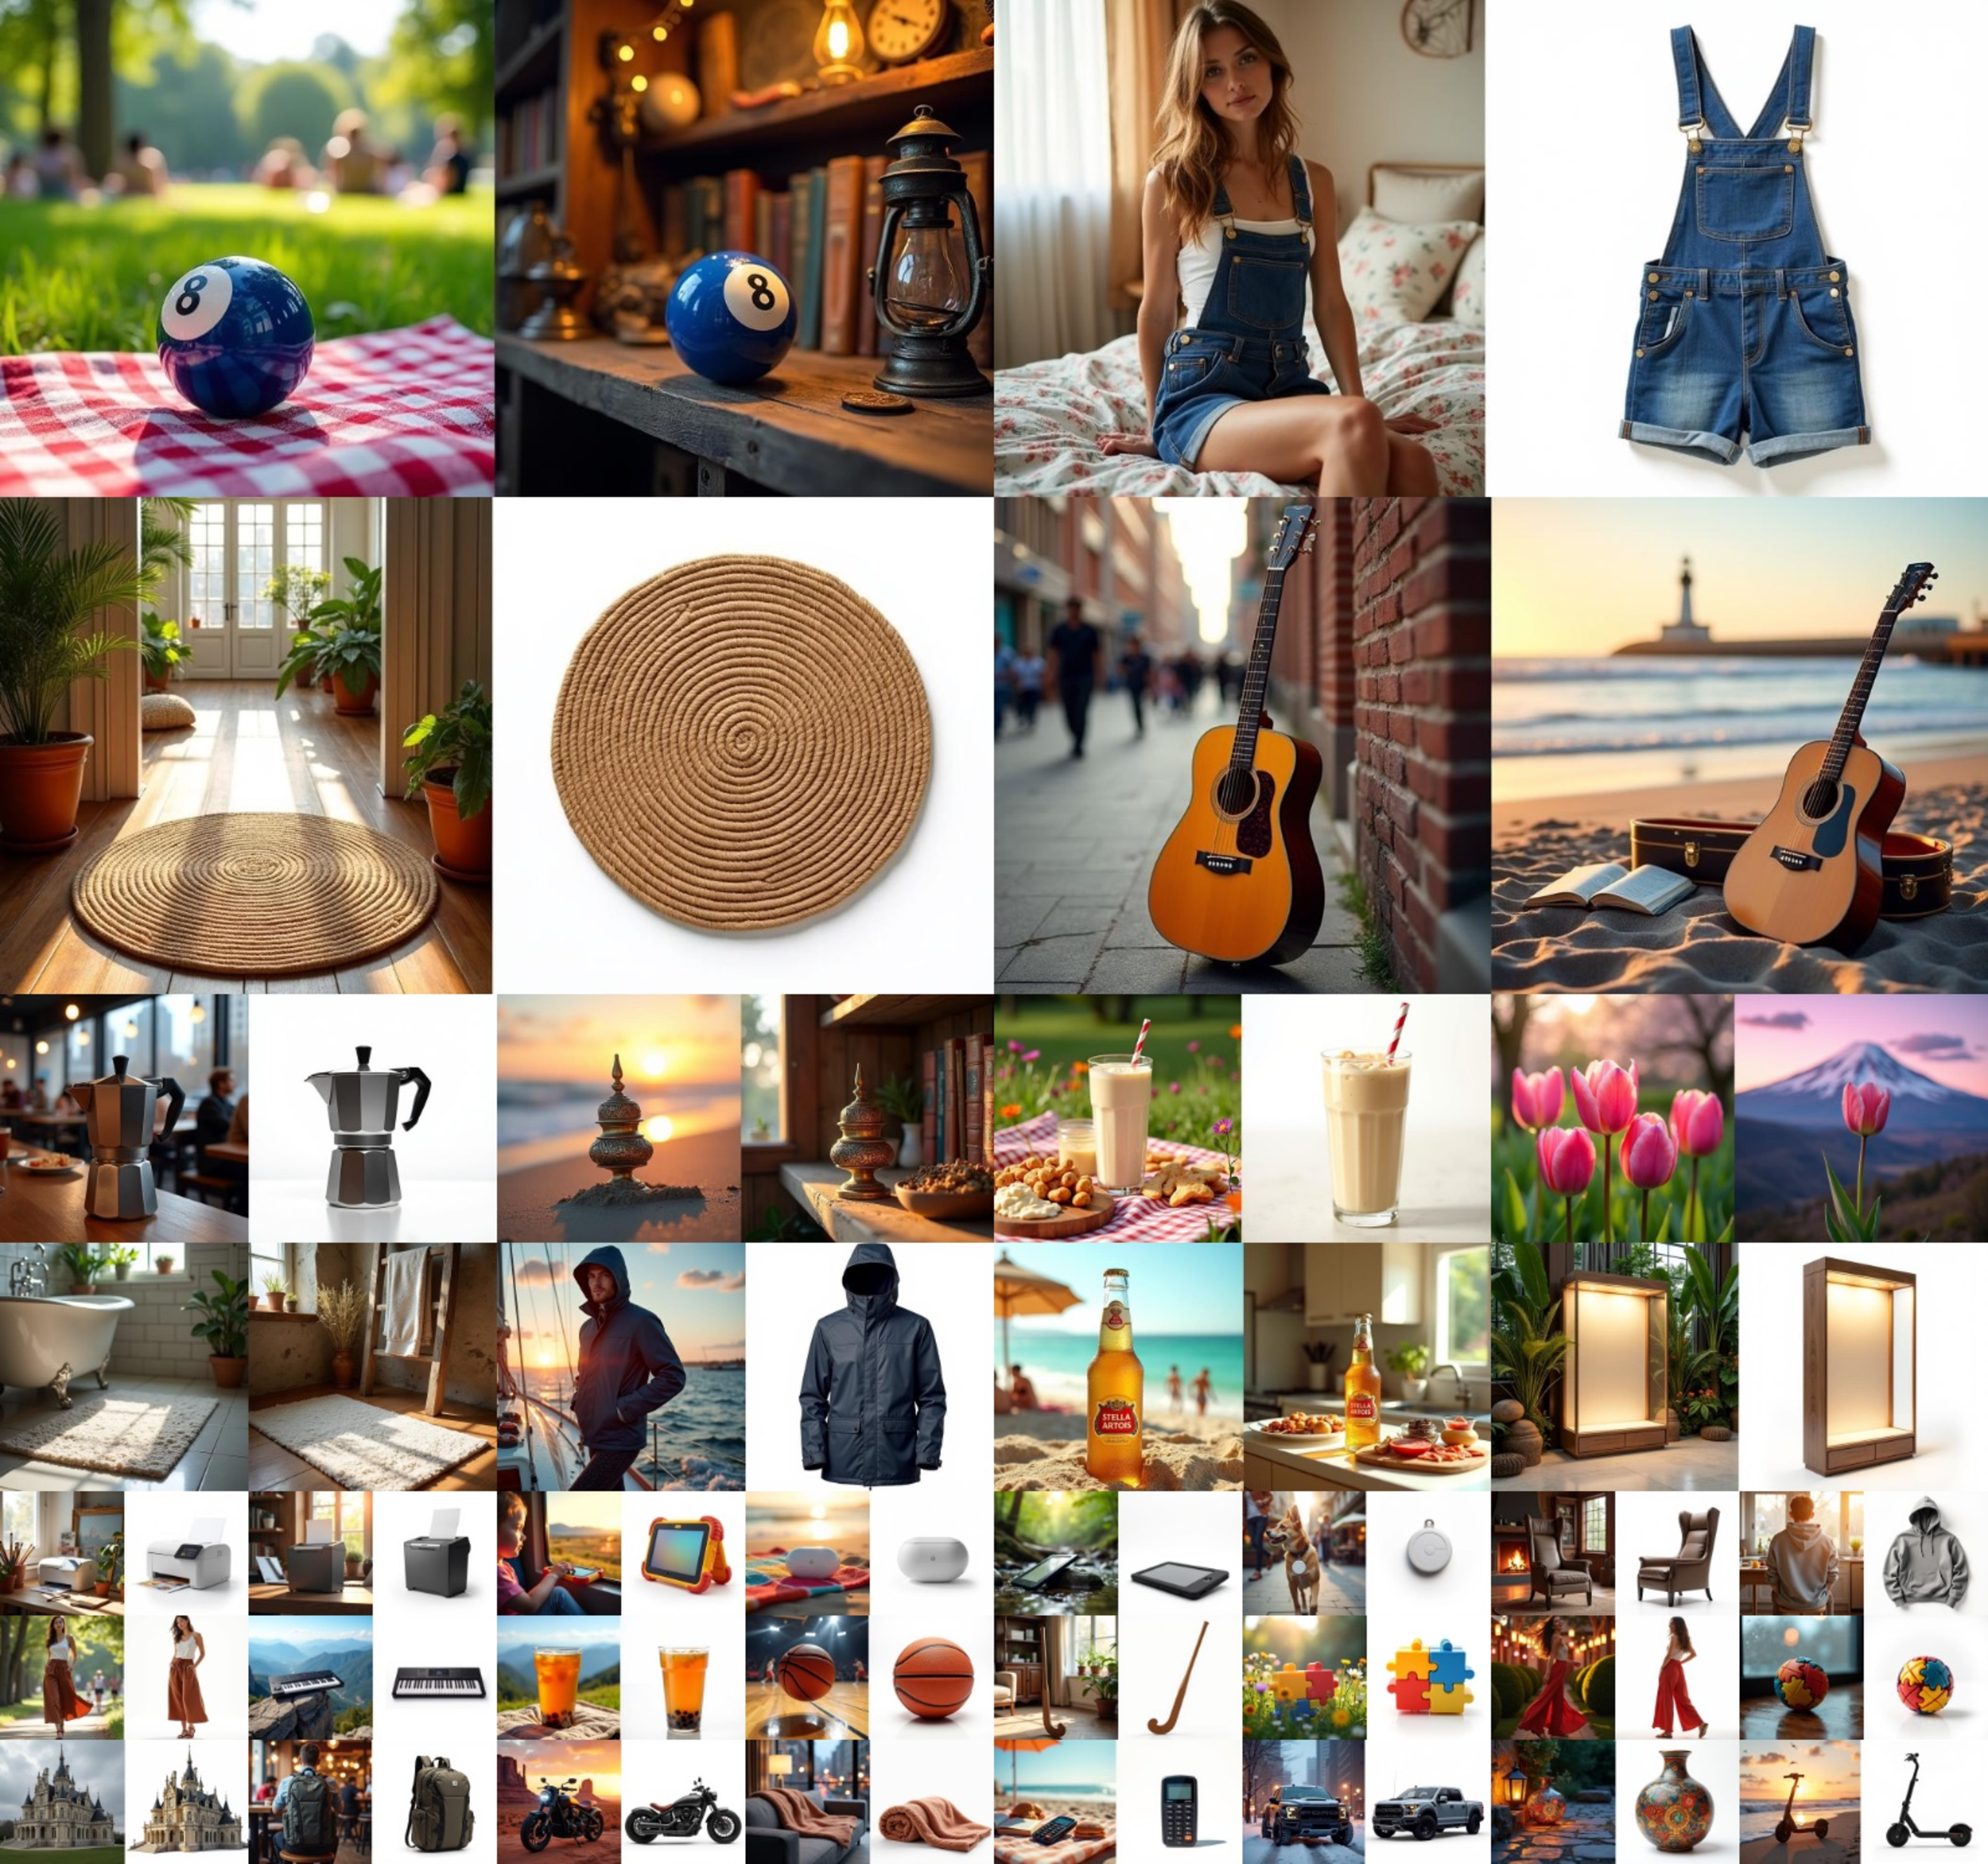
\includegraphics[width=0.8\textwidth]{data2.pdf}
    \caption{Subject200K数据集的部分实例。每个图像对都展示了同一主体在不同位置,角度和光照条件。数据集包括不同主体,如衣服,家具,车辆和动物等。}
    \label{fig5}
\end{figure}
\textbf{任务和基本模型。}我们在两类条件生成任务上评估我们的方法:空间对齐任务和主体驱动的生成。我们的方法建立在 FLUX 的基础上,FLUX是一种用于图像生成的DiT模型。默认情况下,我们使用 FLUX 作为空间对齐的任务生成图像的底模。在主题驱动的生成任务中,我们切换到 FLUX-schenell因为我们观察到它往往会产生更好的视觉质量。\\
\textbf{实现细节。}我们的方法利用 LoRA对基础模型进行微调,默认等级为 4。为了保留模型的原始能力并实现灵活性,在处理非条件标记时默认将 LoRA 等级设置 为 0 进行训练。我们的模型使用批量大小 1 和超过 8 个步骤的梯度累积进行训练(有效批量大小为8).实验在 2 个 NVIDIA H800 GPU(每个 80GB)上进行。对于空间对齐的任务,模型经过 50,000 次迭代的训练, 而主题驱动生成模型经过 15,000 次迭代的训练。\\

\textbf{评估指标。}我们根据空间对齐的任务和主题驱动的生成来评估我们的模型。对于空间对齐的任务,我们评估两个方面:生成质量和可控性。生成质量使用 FID 、SSIM、MAN-IQA 和 MUSIQ来衡量视觉保真度,并使用 CLIP Score\cite{radford2021learning}来衡量语义一致性。为了增强可控性,我们在边缘条件生成中计算提取的边缘图和输入边缘图之间的 FΘ 分数,并计算其他任务的提取的条件图和原始条件图之间的 MSE。\\
对于主题驱动的生成,我们提出了一个标准框架,评估主题特征的保留程度和请求修改的准确性。\\

\textbf{评估准则。}我们对两个数据集进行了评估。对于空间对齐的任务,我们使用大小为 512×512 的 COCO 2017 验证集(5,000 张图像),使用特定于任务的条件和相关的标题作为提示,固定种子为 42。\
对于主题驱动的生成,我们使用 5 个不同的种子,且使用特定的图像作为条件在 750 个文本条件对上进行测试。

\subsection{主要结果}
空间对齐任务如表1\ref{fig:table}所示,我们针对五个空间对齐任务的现有方法全面评估了我们的方法。我们的方法在深度到图像生成方面实现了最高的 FΘ 分数 0.38,显着优于基于 SDΘ.ϸ 的方法 ControlNet和 T2I-Adapter,以及基于 FLUX的 方法ControlNetPro。\
在一般质量指标方面,我们的方法在大多数任务中表现出一致的优越性,在 SSIM\cite{wang2004image}、MAN-IQA\cite{yang2022maniqa} 和 MUSIQ\cite{ke2021musiq}分数中表现出明显更好的性能。对于去模糊和着色等具有挑战性的任务,我们的方法实现了实质性改进:与 Control-NetPro 相比,MSE 分别 降低了 77\% 和 93\%,而 FID 分数在去噪方面从 30.38 提高到11.49。\
CLIP-Score 指标表明我们的方法在所有任务中保持了较高的文本图像一致性,这表明有效保留了语义对齐,同时实现了更好的控制和视觉质量。我们的方法在着色中产生更清晰的细节和更忠实的色彩再现。
\subsection{实验研究}
\textbf{训练数据的影响。}对于主题驱动的生成,我们的模型将主体(例如毛绒玩具或物体)的参考图像和文本描述作为输入,旨在遵循文本指导生成同一主题的新颖图像,同时保留其关键特征。为了验证此前描述的Subjects200K 数据集的有效性,我们比较了该任务的两种训练策略。第一种方法依赖于传统的数据增强,我们对原始图像应用随机裁剪、旋转、缩放以及对比度、饱和度和颜色的调整。\
第二种方法利用我们的Subjects200K 数据集。经过数据增强训练的模型仅学会以最小的变化复制输入条件,如图它只是将玉米卷毛绒玩具放置在明亮的房间环境中,同时保持其精确的外观和姿势。同样,在第二行中,尽管有窗边放置说明,但仍以几乎相同的细节再现了黄色闹钟。 相比之下,我们基于Subjects200K训练模型展示了在遵循文本提示的同时生成不同但一致的主体视图的能力。
\textbf{LoRA 影响。}我们对 Canny 到图像任务的不同 LoRA 等级(1、2、4、8 和 16)进行了广泛的实验。我们的实验表明, 增加LoRA等级通常会提高模型性能,其中LoRA=16在多个方面如图像质量(通过 FID和SSIM测量)、条件控制能力(通过FΘ分数 测量) ,同时保持有竞争力的文本图像一致性 (通过 CLIP-Score 衡量)取得了最佳结果。值得注意的是,即使LoRA等级较小,该模型也表现出一定的竞争力,\
特别是在文本图像对齐方面,它实现了 0.765 的最高 CLIP 分数,显示了我们方法的有效性。
\textbf{深度条件。}FLUX的Transformer架构具有两种不同类型的块:早期块对不同模态标记(文本和图像)采用单独的标准化模块,而后期块则在所有标记之间共享统一标准化。实验表明,将条件信号积分限制为仅这些早期块会导致生成过程的可控性不足。这表明允许条件信号影响整个Transformer对于实现所需的输出至关重要。值得注意的是,这一发现表明主要在早期块中插入条件信号的预览方法在基于 UNet 的架构中有效,但可能无法完全转化为基于 DiT 的模型,如 FLUX。
\section{结论}
OminiControl 使用统一的方法无需额外的模块,为不同任务的扩散模型提供高效参数量的图像调节控制方法,且优于传统方法。提供了一个新的包含超过 200,000 个高质量且主题一致图像的Subjects200K数据集。本篇论文的实验结果证实了 Omini-Control 在扩散模型中的可扩展性和有效性。

\begingroup
    \linespreadsingle{}
    \printbibliography[title={外文翻译参考文献}]
\endgroup
